\documentclass[12pt,a4paper]{article}
\usepackage[UTF8]{ctex}
\usepackage{amsmath,amssymb}
\usepackage{xcolor}
\usepackage{hyperref}
\usepackage{geometry}
\usepackage{graphicx}
\geometry{margin=2.5cm}

\title{Controlled Gates / 受控门}
\author{QuoNic}
\date{}

\begin{document}
\maketitle

\begin{center}
\textbf{Compilation / 编译} | 难度：中级 | 预计时间：10 分钟
\end{center}

\tableofcontents
\newpage

\section{为什么需要？}

受控门是量子计算中的基本门，用于条件操作。

\subsection{经典局限}
\begin{itemize}
  \item 经典逻辑门无法直接用于量子态
  \item 需要量子受控门
\end{itemize}

\subsection{量子优势}
\begin{itemize}
  \item 受控门可以根据控制比特的状态执行不同操作
  \item 是量子纠缠的基础
  \item 是量子算法的核心组件
\end{itemize}

\subsection{实际应用}
\begin{itemize}
  \item 量子纠缠
  \item 量子算法
  \item 量子纠错
\end{itemize}

\section{快速上手}

\begin{verbatim}
from quonic import qgate
from quonic.gates import CX, CZ

# CNOT 门
qgate(CX, 0, 1)  # Control: q0, Target: q1

# CZ 门
qgate(CZ, 0, 1)  # Control: q0, Target: q1
\end{verbatim}

\textbf{预期输出}：
\begin{verbatim}
(CX gate applied)
(CZ gate applied)
\end{verbatim}

\section{原理详解}

\subsection{电路图}

\begin{center}
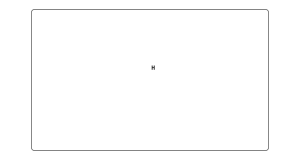
\includegraphics[width=0.6\textwidth]{../../images/controlled_circuit.svg}
\end{center}

\subsection{数学推导}

CNOT 门：
\begin{equation}
\text{CNOT} = |0\rangle\langle 0| \otimes I + |1\rangle\langle 1| \otimes X
\end{equation}

CZ 门：
\begin{equation}
\text{CZ} = |0\rangle\langle 0| \otimes I + |1\rangle\langle 1| \otimes Z
\end{equation}

\subsection{几何解释}

受控门在 Bloch 球上根据控制比特的状态执行不同操作。如果控制比特是 $|1\rangle$，则对目标比特执行操作。

\section{代码详解}

\begin{verbatim}
from quonic import qgate
from quonic.gates import CX, CZ, CY

# CNOT 门: Control q0, Target q1
qgate(CX, 0, 1)

# CZ 门: Control q0, Target q1
qgate(CZ, 0, 1)

# CY 门: Control q0, Target q1
qgate(CY, 0, 1)
\end{verbatim}

\section{进阶用法}

\subsection{场景 1：多控制门}

\begin{verbatim}
from quonic import qgate
from quonic.gates import CCX

# Toffoli 门: Control q0, q1; Target q2
qgate(CCX, 0, 1, 2)
\end{verbatim}

\subsection{场景 2：受控旋转门}

\begin{verbatim}
from quonic import qgate
from quonic.gates import CRz
import math

# 受控 Rz 门
qgate(CRz(math.pi/4), 0, 1)
\end{verbatim}

\section{适用场景}

\subsection{量子纠缠}

受控门用于创建量子纠缠。例如，CNOT 门可以创建 Bell 态。

\subsection{量子算法}

受控门是许多量子算法的核心组件。例如，QFT、QPE 等都需要受控门。

\section{常见问题}

\subsection{受控门和普通门有什么区别？}

受控门根据控制比特的状态执行不同操作，普通门无条件执行。

\subsection{受控门有哪些类型？}

常见的受控门包括：CNOT、CZ、CY、CCX（Toffoli）、CSWAP（Fredkin）等。

\section{学习路径}

\subsection{前置知识}
\begin{itemize}
  \item 量子门
  \item 量子比特
  \item 量子测量
\end{itemize}

\subsection{继续学习}
\begin{itemize}
  \item 量子纠缠
  \item 量子算法
  \item 量子纠错
\end{itemize}

\section{完整示例代码}

\subsection{示例 1：基本受控门}

\begin{verbatim}
from quonic import qgate
from quonic.gates import CX

qgate(CX, 0, 1)
\end{verbatim}

\section{下载}

\begin{itemize}
  \item [controlled.py](https://github.com/ChrisLee0721/QuoNic/blob/main/examples/controlled/controlled.py)
\end{itemize}

\end{document}
